%!TEX program = pdflatex
%!BIB program = bibtex

\documentclass[a4paper,11pt]{article}
\usepackage{graphicx}
\usepackage{amsmath, amsthm, amssymb} %better typesetting of mathematical expressions, theorems, additional symbols
\usepackage{booktabs} %fixltx2e
\usepackage[flushleft]{threeparttable}
\usepackage{tabularx}
% \usepackage[capposition=top]{floatrow}
\usepackage{caption}
% \captionsetup[measuredfigure]{labelformat=empty}
% \usepackage{bm}
% \usepackage{subcaption}
\usepackage{epstopdf} % not supported by xelatex
% \usepackage{fullpage}
% \usepackage{enumerate}
\usepackage{authblk}
\usepackage[T1]{fontenc}
\usepackage{inputenc}
\usepackage{lmodern}
% \usepackage{fontspec}
\usepackage{lscape}
\usepackage[round]{natbib} %standard package for bibliography
\usepackage{multirow}
% \usepackage[figuresleft]{rotating}
\usepackage[dvipsnames]{xcolor}
\usepackage{colortbl} % color table
\usepackage{geometry}
% \usepackage{hyperref} %hyperlink support
% \hypersetup{pdfstartview={XYZ null null 1.00},bookmarksnumbered, hypertexnames=false, colorlinks=true, linkcolor=BrickRed, citecolor=MidnightBlue, urlcolor=MidnightBlue} % zoom: default screen; numbers for bookmarks

%
%
%\usepackage{parskip}
\usepackage[nolist]{acronym}
\usepackage{longtable}
\usepackage{setspace}

\acrodef{bic}[BIC]{Bayesian Information Criterion}
\acrodef{bma}[BMA]{Bayesian Model Averaging}
\acrodef{cbf}[CBF]{Conditional Bayes Factor}
\acrodefplural{cbf}[CBFs]{Conditional Bayes Factors}
\acrodef{cswd}[CSWD]{Credit Suisse Wealth Databook}
\acrodef{dina}[DINA]{Distributional National Accounts}
\acrodef{efw}[EFW]{Economic Freedom of the World}
\acrodef{fdi}[FDI]{Foreign Direct Investment}
\acrodefplural{fdi}[FDIs]{Foreign Direct Investments}
\acrodef{gdp}[GDP]{Gross Domestic Product}
\acrodef{gfdd}[GFDD]{Global Financial Development Database}
\acrodef{hbs}[HBS]{Household Balance Sheet}
\acrodef{ivbma}[IVBMA]{Instrumental Variable Bayesian Model Averaging}
\acrodef{lis}[LIS]{Luxembourg Income Study}
\acrodef{oecd}[OECD]{Organisation for Co-operation and Development}
\acrodef{pip}[PIP]{Posterior Inclusion Probability}
\acrodefplural{pip}[PIPs]{Posterior Inclusion Probabilities}
\acrodef{pmp}[PMP]{Posterior Model Probability}
\acrodef{swiid}[SWIID]{Standardized World Income Inequality Database}
\acrodef{uip}[UIP]{Unit Information Prior}
\acrodef{uk}[UK]{United Kingdom}
\acrodef{us}[US]{United States}
\acrodef{wals}[WALS]{Weighted-average Least Squares}
\acrodef{wb}[WB]{World Bank}
\acrodef{wid}[WID]{World Inequality Database}
\acrodef{wiid}[WIID]{World Income Inequality Database}


%
%

\setlength\parindent{34pt}
\onehalfspacing
\title{Finance and Income Inequality - panel BMA approach\thanks{The author acknowledges support from Charles University Research Centre program No. UNCE/HUM/035}}
% \author[a]{Roman Horvath}
\author[a]{Jan Mares\footnote{\footnotesize Corresponding author's address: IES FSV UK, Opletalova 26, 110 00, Praha 1; \textbf{e-mail:janxmares@gmail.com}}}
\affil[a]{Charles University, Prague}


%\renewcommand\Authands{ and }
\date{\today}

\begin{document}


\clubpenalty 9999 % no orphans (typographic properties)
\widowpenalty 9999 % no widows (typographic properties)
\def\sym#1{\ifmmode^{#1}\else\(^{#1}\)\fi} % shortcut for Stata tables

\maketitle

\thispagestyle{empty}
\begin{abstract}
    We investigate the impact of financial development on income inequality differentiating between depth, efficiency and access to financial markets and institutions. We apply panel Bayesian model averaging framework to address model uncertainty to reveal that financial development has complex influence on the income distribution within countries. The access to and efficiency of banking decrease income inequality. The size of the markets has no influence on overall income inequality, but contributes to the increasing top income shares. Moreover, unemployment along with investment into non-tangible assets increase income inequality while higher redistribution and physical capital investment imply lower levels of inequality.
\end{abstract}

\bigskip

\begin{tabular}{p{0.25\hsize}p{0.6\hsize}} %0.15
\textbf{Keywords:} & Income inequality, finance, Bayesian model averaging
\end{tabular}

\bigskip

\begin{tabular}{p{0.25\hsize}p{0.6\hsize}}
\textbf{JEL Codes:} & D31, E21\\
\end{tabular}

\clearpage
\setcounter{page}{1}

\section{Introduction}
% \label{sec:intro}
% Financial development alters how much are economic opportunities depend on the individual skills, family endowments, social status or political connections. Individual depend on financial system to provide loans to start new business, attain education

Finance captures the capacity of financial intermediaries and markets to screen investment opportunities, monitor the debtors who were provided funding, as well as pooling and management of risk. With inequality, we focus in the paper on the inequality in the distribution of income. Arguably, the literature discusses other concepts of inequality, e.g. intergenerational persistence of relative income differences or equality of opportunity \citep{demirgucc2009finance}.

\citet{claessens2007finance} argue that although deeper financial systems generally provide better opportunities of access to finance, the relationship is not universal.

The average income inequality rose across \ac{oecd} by 1.4 percentage points \citep{oecd2013crisis}.

\section{Related literature}
% \label{sec:literature}
The research in the area of financial development and income inequality is well established. \citet{demirgucc2009finance}, \citet{claessens2007finance}, and more recently \cite{de2017finance} provide extensive reviews of the topic. A similar theme emerges in all three papers. The implications from theoretical contributions provide conflicting predictions about the relationship and empirical results bring evidence for both positive and negative effect. Although majority of the papers point towards finance tightening the distribution of income this results is not universal with some papers suggesting the opposite while other stress potential non-linearities.

A key divide appears between the effect of financial development on extensive and intensive margin. The extensive margin captures the extend to which individuals, who had not been using financial services before, gain access. On the other hand, the intensive margin describes growing use of finance by the agents who had already been using it before \citep{demirgucc2009finance}. Financial development on the extensive margin might lead to more equal opportunities and outcomes. Access to credit by previously disadvantaged groups allows human capital accumulation \citep{galorzeira1993income, galormoav2004, braunetal2019}, formation and growth of new firms \citep{evans1989estimated,banerjeenewman1990}, with more evenly distributed economic opportunities as a result\footnote{Having similar economic opportunities might decrease the cross-generational inequality, by diminishing the effect of e.g. parental wealth. Depending on the innate abilities and talents of the individuals, however, it may increase the inequality of income within every generation at the same time.}.

On the contrary, intensive margin of financial development might disproportionately benefit the rich who may leverage financial services for their further benefit or to protect their existing rents. \citet{GreenwoodJovanovic1990} present a model where the finance is the key driver of inequality and the welfare gains accrued by the incumbents - primarily the rich - in the initial development stage. With time, more agents meet the fixed costs of joining the financial intermediaries and they enjoy higher returns. Consequently, the efficiency of resource allocation also increases, which enhances growth and reduces inequality. \citet{perotti2007investor} present a framework based on political economy. They argument depends on a lobby for lower investor protection to prevent entrance of the new competitors. The politicians require higher bribe from the lobbyist the greater is their accountability for policy decisions. Thus, with increasing accountability, investor protection strengthens and spurs market entry and competition. The authors examine their prediction in a cross-section and show that better investor protection correlates with larger entry rates and higher firm density in more financially intensive sectors\footnote{In addition, they show that the most important factor of accountability is not the formal measure of democratic institutions, but newspaper readership which they interpret as broad awareness of policy choices and their outcomes.}. 

Financial development may also have indirect effect on income inequality through economic growth. \citet{townsendeueda2006} model how finance interacts with production and allocation of credit. If increased use of finance increases the demand for low- relatively to the high-skilled workers, then it may have equalizing consequences for income distribution. Empirical evidence by \citet{beck2010big} show that bank deregulation and increased competition in loan provision in the \ac{us} primarily benefited the workers with income below the median. Similarly, \citet{delis2014} provide evidence of bank deregulation and liberalization tightening the income distribution, although this effect is only present in countries with high-quality institutions. They attribute the effect to the changes in labour market conditions and relatively higher wages and working hours of the low-skilled workers following the reforms. 

A set of distinct papers explores the relationship between inequality and growth while stressing financial markets imperfections driving the outcomes. Income inequality and growth may intersect through varying channels. Accumulation of savings, unobservable effort, and investment project size favor the prediction of growth inducing inequality. Negative impact of inequality on human capital accumulation, entrepreneurial activity provide argument for the opposing view. 
\citet{van2018inequality} report how income inequality in the \ac{us} has different implications for the future income growth of the rich and the poor. High inequality seems to hurt the prospects of the poor while the top of the distribution is unaffected. The rich thus disproportionately benefit from higher inequality as their subsequent income exhibit faster growth. The authors attribute this effect to the political channel the rich use to lobby in favor of the policies which support their economic interests. Preferences of the rich are ultimately more likely to determine public policy than the preferences of the majority \citep{gilens_page_2014}. High inequality together with a credit constraint and rich driving the political process results in low government spending and lasting inequality.

The literature does not converge on the conclusions even in the empirical cross-country and panel data studies. The papers link higher levels of financial development with lower levels of inequality \citep{beck2007finance, hamori2012, gimet2011closer, kunieda2014finance}\footnote{For an extended list, we refer to \citet{de2017finance}.}. On the other hand, several other estimate a growth inducing effect of finance \citep{Jaumotte2013, jauch2016financial, de2017finance}. Finally, some authors claim there the relationship might be non-linear, conditional on a threshold value of financial development \citep{kim2011nonlinearity,tan2012nonlinear} or institutional quality \citep{LawSingh2014, delis2014}.

Three papers are the closest to ours, each in a different respect. First, \citet{de2017finance} examine different dimensions of finance on income inequality. Their results suggest that financial development, financial liberalization, and banking crises all increase pre-tax income inequality within countries. Additionally, they show that the effect of financial liberalization is conditional on democratic accountability. Higher accountability mitigates the impact of liberalization on inequality. On the contrary, the financial development, proxied by the credit to GDP ratio, has inequality increasing effect irrespective of the institutional background. Second, \citet{naceurzhang2016} take similar approach in considering multiple dimensions --- the access, efficiency, and stability of the financial sector, although not examining the indicators simultaneously.  Third, \citet{furceri2019robust} apply \ac{wals} to identify robust determinants of income inequality. Their approach mirrors ours in accounting for model uncertainty in the estimation. Their focus is more general rather than focused primarily on finance. We provide synthesis and extension to these papers in providing more detailed view on the link between finance in shaping income inequality and examining multiple measures of inequality while specifically identifying the determinants of top income shares along with the determinants of the overall income distribution\footnote{Captured by income Gini index}.

% An exemption from focus solely on the size of financial sector is the study by \citet{naceurzhang2016} which applies a similar approach to ours, taking into consideration the access, efficiency, and stability of the financial sector. However, there are severe limitation to their study. First, their coverage does not correspond to the availability of the data. Second, they do not account for the different dimensions of finance simultaneously and always use a single indicator of development at a time. Third, they do not explicitly differentiate between the banking sector and financial markets. We provide a more detailed as well as more robust picture of the financial development effect on finance in these dimensions.

% \citet{de2017finance} examine different dimensions of finance on income inequality. Their results suggest that financial development, financial liberalization, and banking crises all increase market income inequality within countries. Additionally, they show that the effect of financial liberalization is conditional on democratic accountability. The higher the accountability, the less severe is the negative impact of liberalization on inequality. On the contrary, the financial development, proxied by the credit to GDP ratio, has inequality increasing effect irrespective of the institutional background.

% \citet{furceri2019robust} apply WALS to identify robust determinants of income inequality. They are the closest paper to ours since they account for model uncertainty in the estimation. Their focus if more general rather than on finance specifically. Out work offers more detailed contribution in terms of the role of finance in shaping income inequality. On the top of that, we differ from their analysis by examining multiple measures of inequality and specifically identifying the determinants of top income shares along with the determinants of the overall income distribution represented by income Gini index. We provide further evidence in all these dimensions.

%
%
%
%
%

\section{Data}
The key variable in the paper is the measure of income inequality. We want to examine how financial development affects income inequality and whether the effect might by different at the top quantiles of income distribution. As the overall measure of income inequality, we rely the after-tax Gini coefficient from \ac{swiid} by \citet{Solt2019}, which is a standard resource in the literature\footnote{There are alternative sources of for Gini coefficient, e.g. \ac{wiid} or \ac{lis}, but each of them brings limitations in terms of comparability or coverage.}. Its critical advantage lies in the widespread coverage across countries and time and a unified methodology which provides a reasonable level of comparability. It typically takes values in the interval between 0 and 100 where the former suggests perfect equality (everyone in the economy enjoys the same income) and the latter perfect inequality (all the income goes to only a single unit). We depart from existing papers slightly in considering the after-tax rather than the before-tax income distribution as a dependent variable. 

To explore the relationship in the top part of the distribution, we choose top income share from \ac{wid}\footnote{The methodology and guidelines to database are provided by \citet{alvaredo2016distributional}.}. The surveys suffer from well-known issues of underrepresentation of the top income earners and the distortions resulting from self-reported character of the data. This can influence not only the top income shares resulting from survey data, but also distortions in the overall measures of inequality. The data in \ac{wid} make use of income tax records in individual countries and the derived shares obtained using consistent methodology of \ac{dina} are arguably more reliable relative to the survey-based measures which are the primary source of majority estimates of income distributions. 

The data spans from 2000 to 2014. We follow the literature \citep{dabla2015causes,de2017finance} and average both the inequality measure (dependent variable) and the potential determinants (independent variables) across three year intervals. There are important reasons for looking at the averages than observation in individual years. Annual macroeconomic data are subject to fluctuations and the data on income inequality is noisy \citet{delis2014}. Averaging should diminish the level of noise. On the top of that, the variables at the center of our analysis, e.g. stock market capitalization or credit to \ac{gdp}, are likely to be affected by the business cycles and volatile on the yearly basis. Similar argument holds for top income shares, as they depend, among other things, on the bonuses paid out each year and capital income. We want to explore the long-term rather than the short-term relationship and that guides the choice of averaged data. Faced against the trade-off between length of the averaging periods and available observations in the time dimension, we take a compromise of three years in contrast to the literature, where generally the 5-year intervals apply. The availability of financial development indicators limits the analysis to a period from 2000 onward and we prefer to keep at least 5 unique time periods to just three under the case of 5-year average\footnote{Nevertheless, we run the estimation with 5-year averages of data as a robustness check and find no critical qualitative differences compared to the baseline.}.

Table \ref{tab:ineq} report the summary statistics and correlations between the income inequality variables.

\begin{table}[ht!]
    \small
    \caption{Summary statistics of inequality variables}
    \label{tab:ineq}
    \centering
       \begin{tabular}{lrrrr}
        \toprule
        Variable & Mean & St. Dev. & Min & Max \\
        After-tax Gini (SWIID) & & & & \\
        Top 10\% income share & & & & \\
        Top 1\% income share & & & & \\
        \bottomrule
    \end{tabular}
\end{table}

\cite{roineetal2009}, \citet{furceri2019robust} for the determinants of income inequality.

\citet{nolan2019drivers} bring a survey of the literature on determinants of inequality, summarizing the complexity of the inequality dynamics. They stress that many of the determinants are interlinked which implies difficulty in assigning precise effects to individual drivers of inequality. Additionally, they encourage complementary individual country case studies to support the finding of the general cross-country estimates.

Both theoretical and empirical studies leave out the issue of importing the financial services from abroad. We include financial globalization from KOF among our control variables.

% % \label{sec:data}
% \begin{figure}
%     \caption{Gini Coefficient and Efficiency of Financial Institutions}
%     \label{fig:ginifie}
% 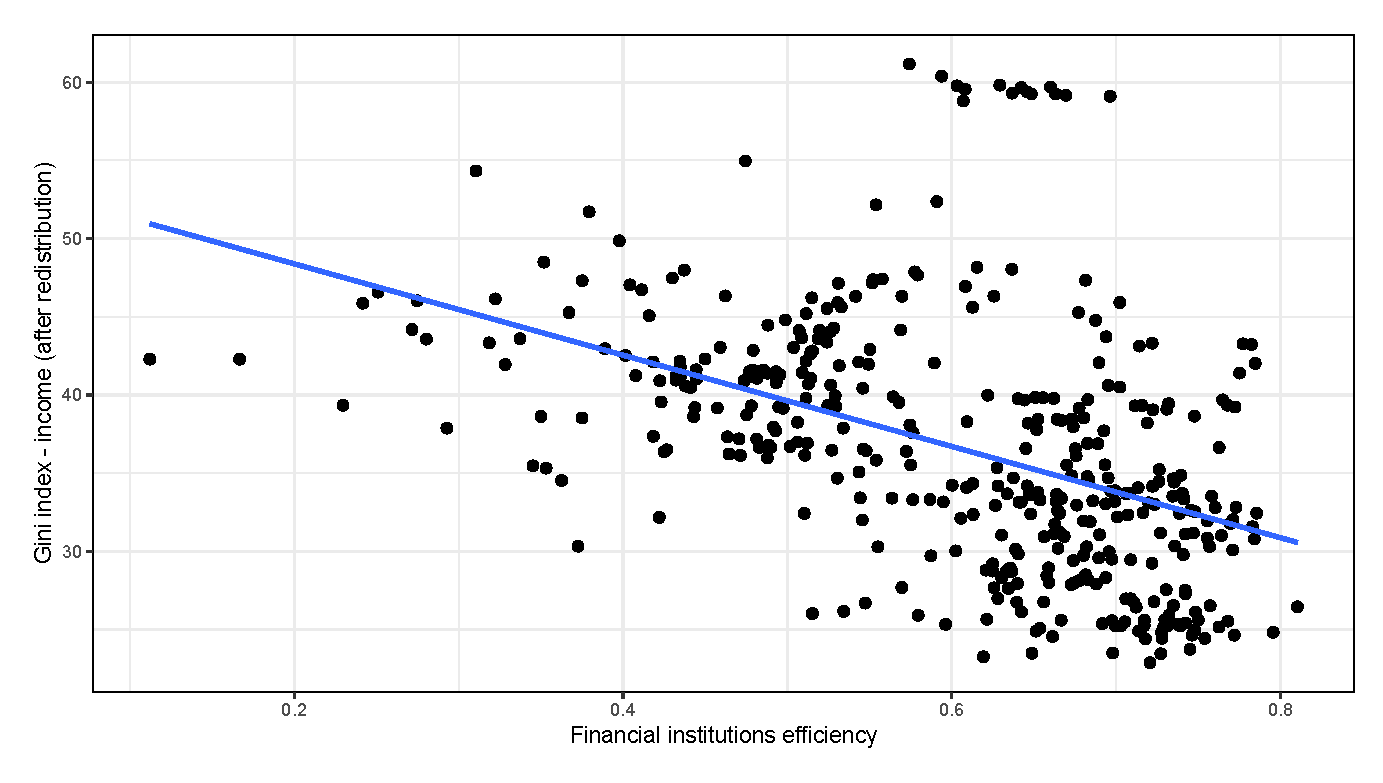
\includegraphics[width=\textwidth, keepaspectratio]{figures/FIEGiniNet}
% \end{figure}

% \begin{figure}
%     \caption{Gini Coefficient and Access to Financial Institutions}
%     \label{fig:ginifia}
% 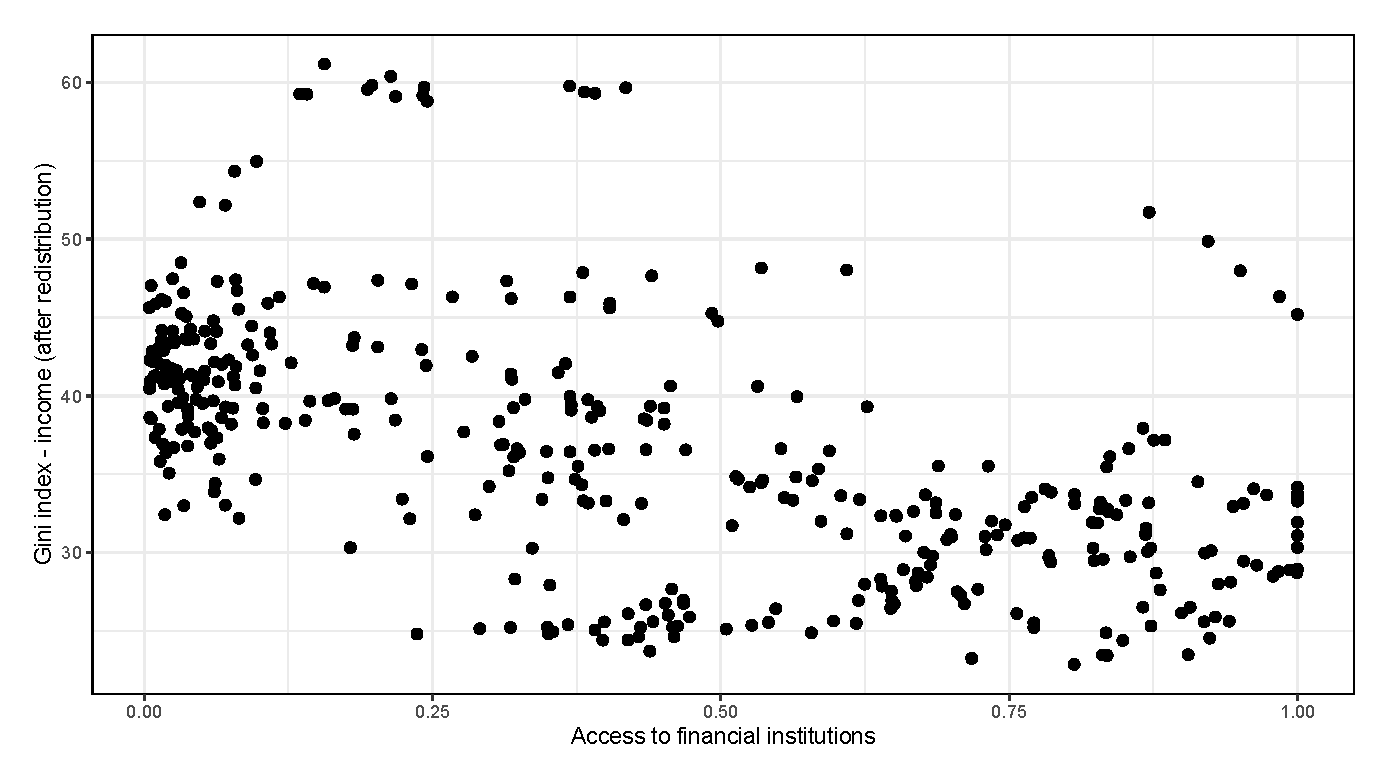
\includegraphics[width=\textwidth, keepaspectratio]{figures/FIAGiniNet}
% \end{figure}

% \begin{figure}
%     \caption{Gini Coefficient and Depth of Financial Institutions}
%     \label{fig:ginifid}
% 
\includegraphics[width=\textwidth, keepaspectratio]{figures/FIDGiniNet}
% \end{figure}

% \begin{figure}
%     \caption{Gini Coefficient and Depth of Financial Markets}
%     \label{fig:ginifmd}
% 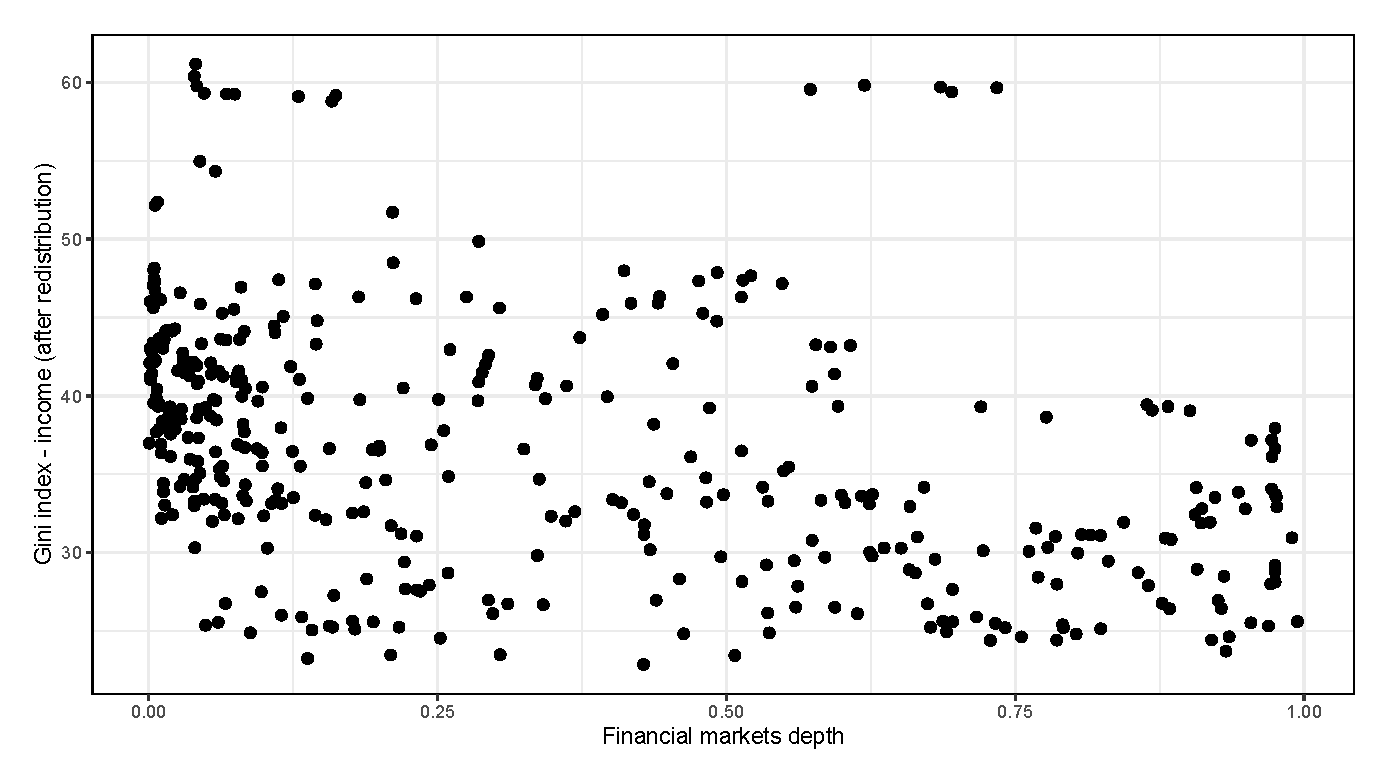
\includegraphics[width=\textwidth, keepaspectratio]{figures/FMDGiniNet}
% \end{figure}

% \begin{figure}
%     \caption{Gini Coefficient and Government Expenditures}
%     \label{fig:ginigovexp}
% 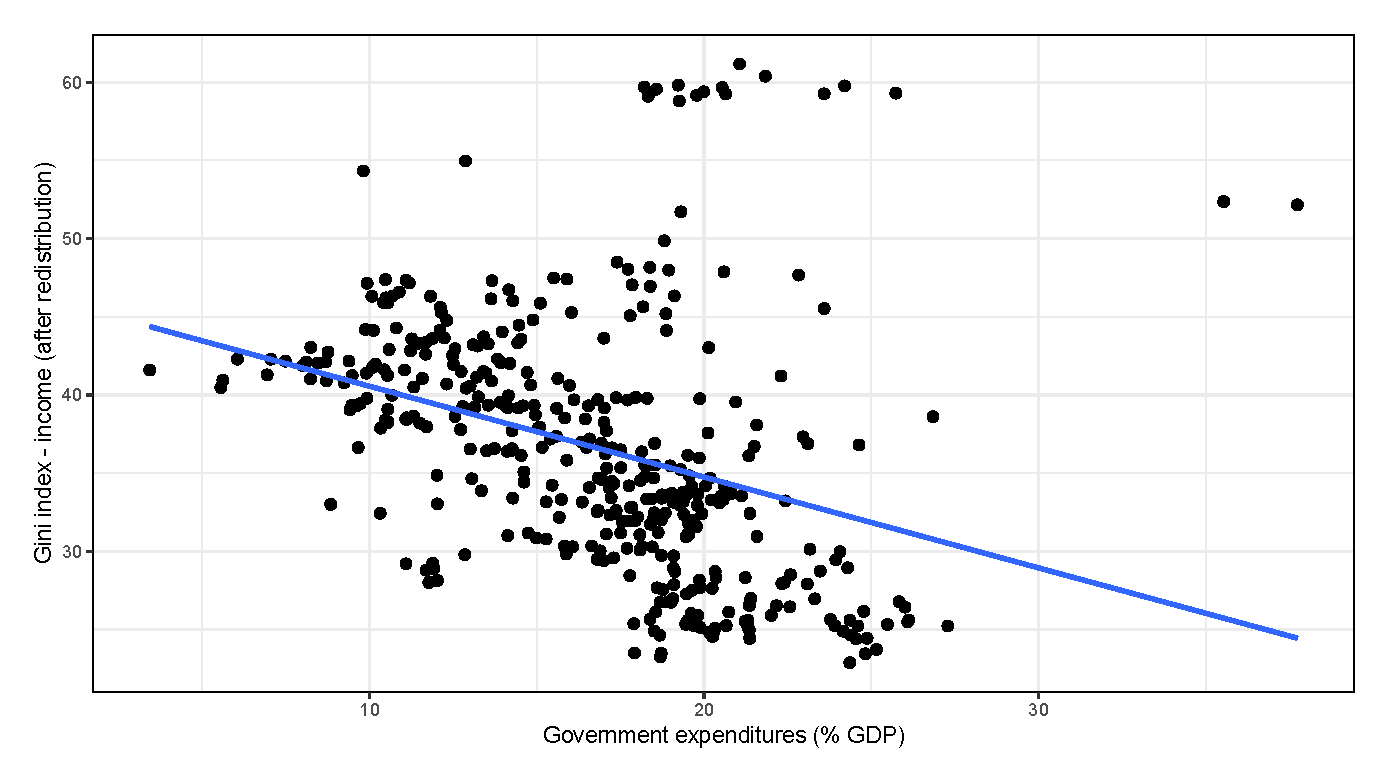
\includegraphics[width=\textwidth, keepaspectratio]{figures/GovExpGiniNet}
% \end{figure}

% \begin{figure}
%     \caption{Gini Coefficient and Mortality}
%     \label{fig:ginimort}
% 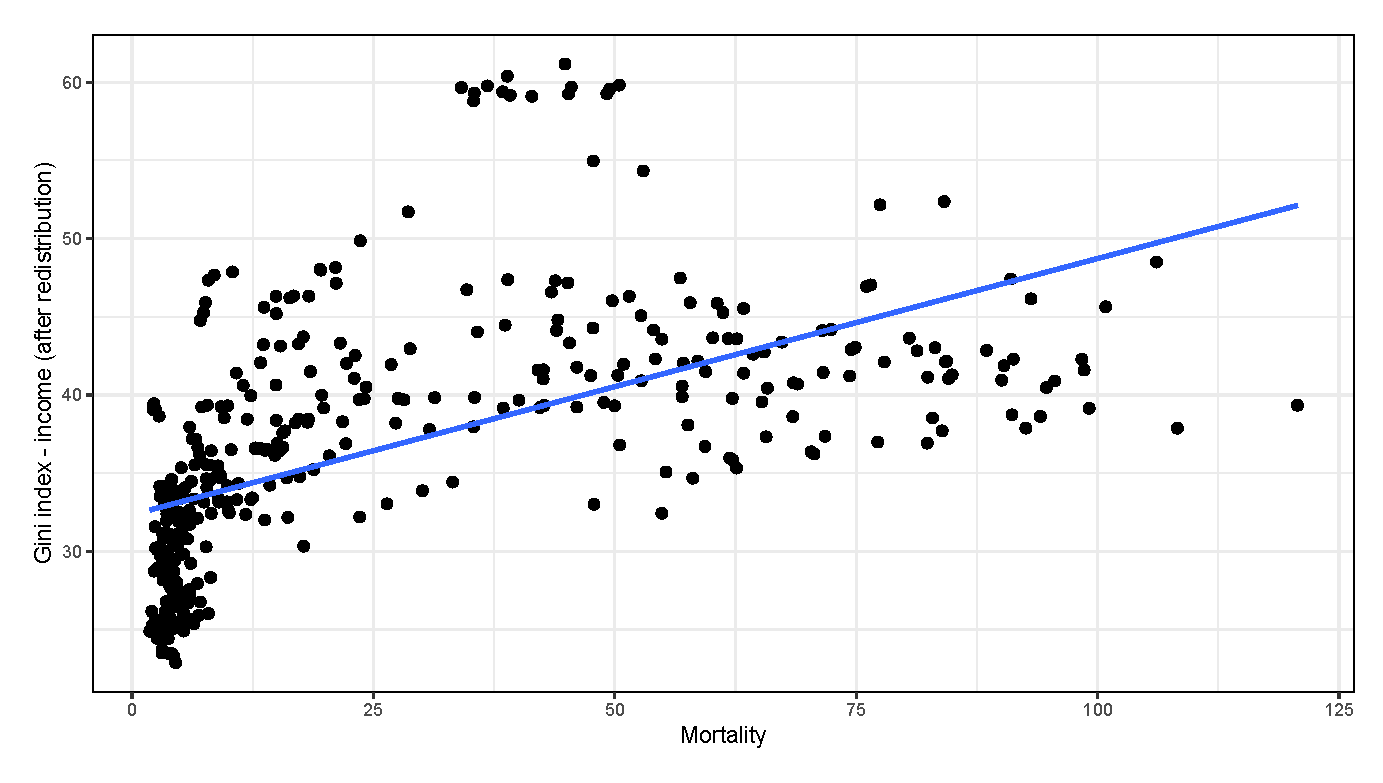
\includegraphics[width=\textwidth, keepaspectratio]{figures/MortGiniNet}
% \end{figure}

% \begin{figure}
%     \caption{Gini Coefficient and \ac{gdp} per capita}
%     \label{fig:ginigdp}
% 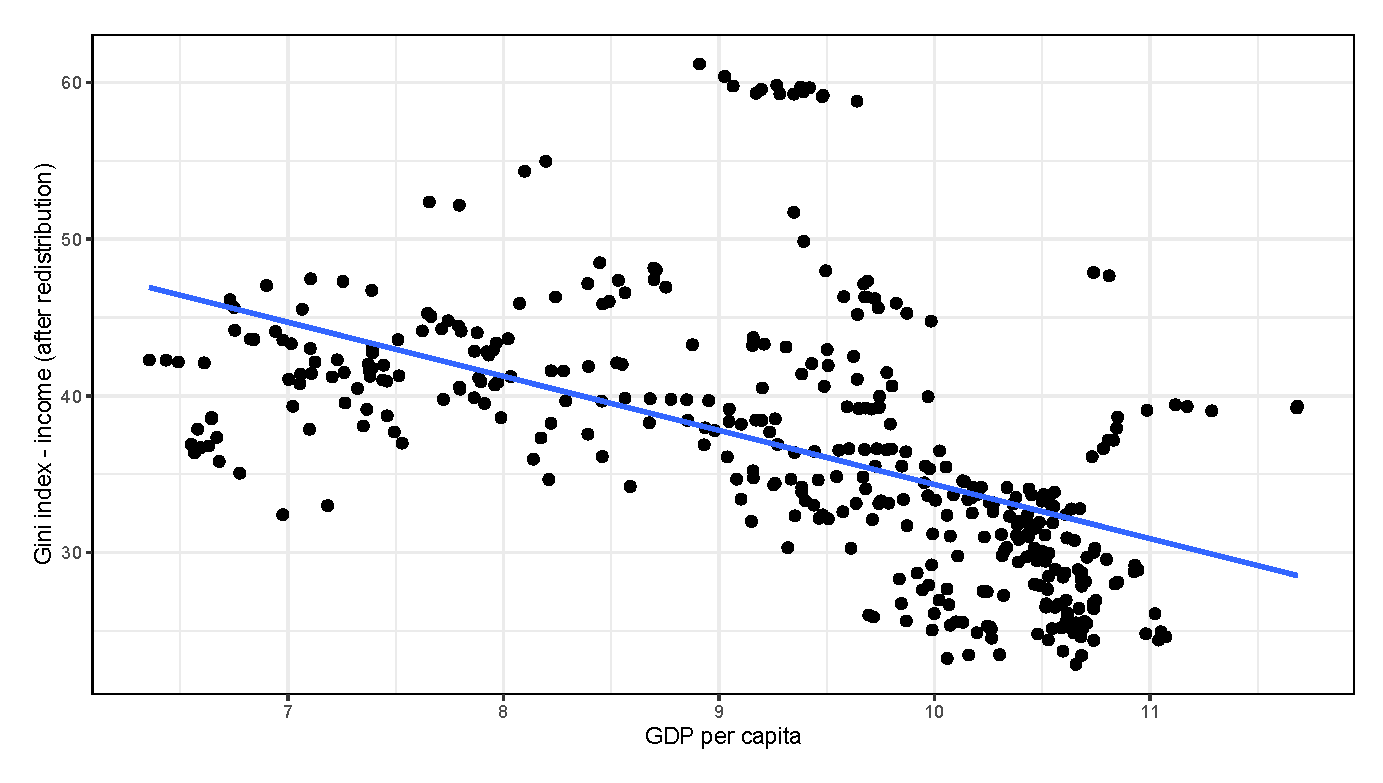
\includegraphics[width=\textwidth, keepaspectratio]{figures/GDPGiniNet}
% \end{figure}

% \begin{figure}
%     \caption{Gini Coefficient and Rule of Law}
%     \label{fig:ginirule}
% 
\includegraphics[width=\textwidth, keepaspectratio]{figures/RuleLawGiniNet}
% \end{figure}

% \begin{figure}
%     \caption{Gini Coefficient and Inflation}
%     \label{fig:giniinfl}
% 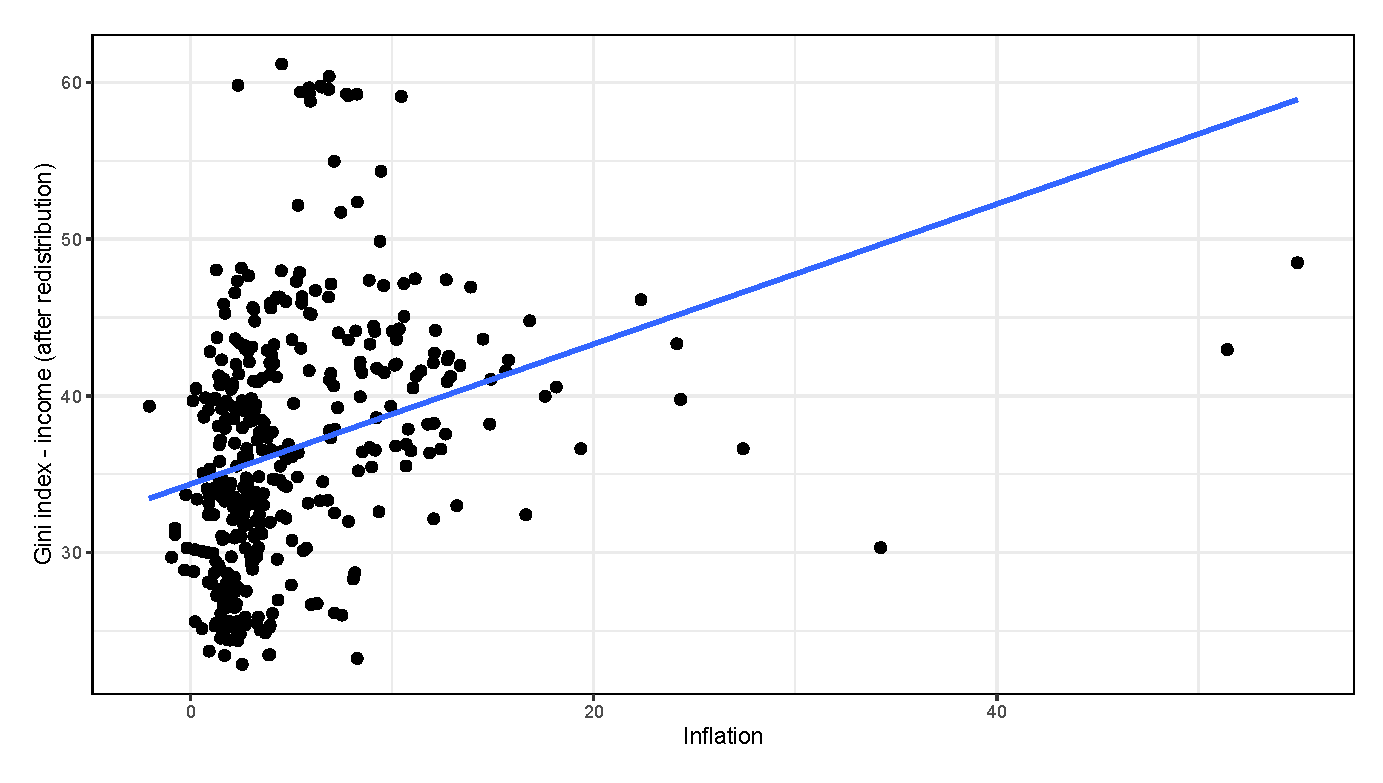
\includegraphics[width=\textwidth, keepaspectratio]{figures/InflGiniNet}
% \end{figure}

% \begin{figure}
%     \caption{Gini Coefficient and Equipment Investment}
%     \label{fig:giniequipi}
% 
\includegraphics[width=\textwidth, keepaspectratio]{figures/EquipIGiniNet}
% \end{figure}

% \begin{figure}
%     \caption{Gini Coefficient and Trade Openness}
%     \label{fig:ginitrade}
% 
\includegraphics[width=\textwidth, keepaspectratio]{figures/TradeOpenGiniNet}
% \end{figure}

% \begin{figure}
%     \caption{Gini Coefficient and Financial Development Indicators}
% 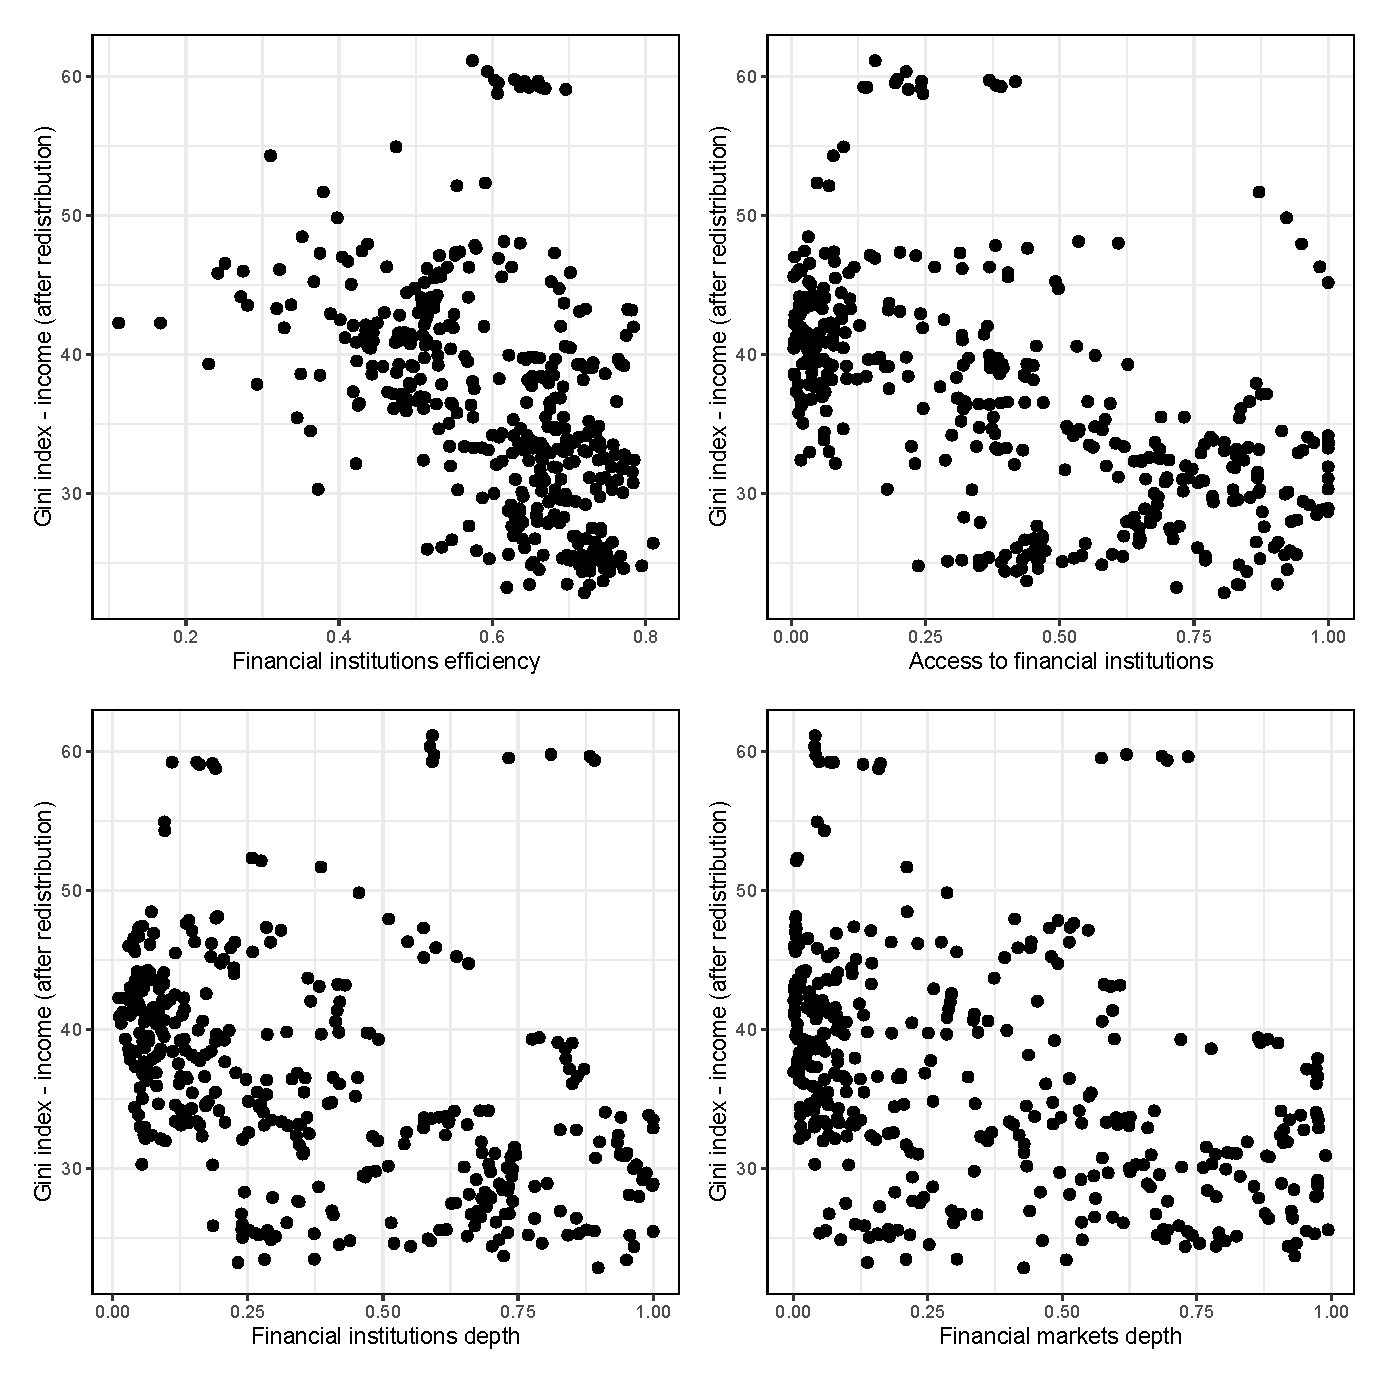
\includegraphics[width=\textwidth, keepaspectratio]{figures/plots_findev_gini}
% \end{figure}

% %
% %

% \begin{figure}
%     \caption{Gini Coefficient and Efficiency of Financial Institutions}
% 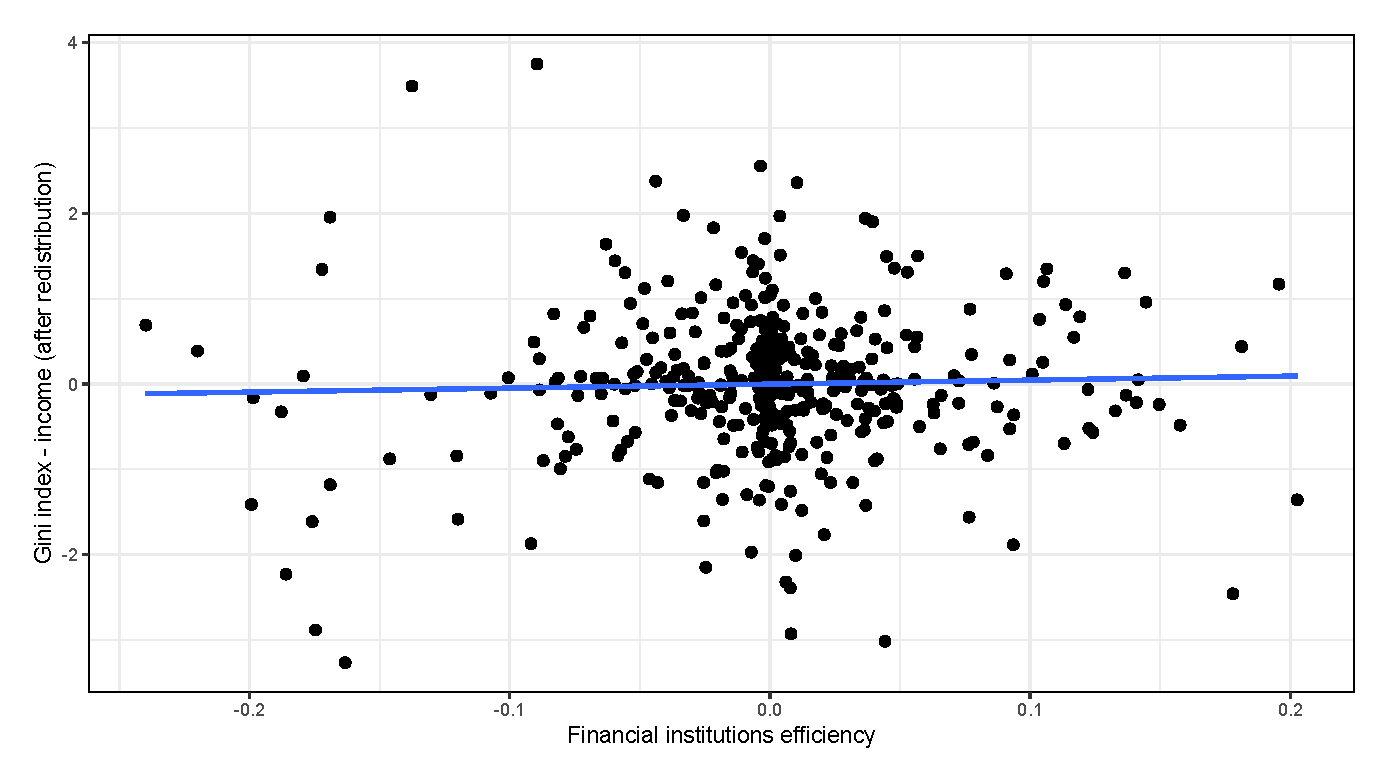
\includegraphics[width=\textwidth, keepaspectratio]{figures/FIEGiniNet_dm}
% \end{figure}

% \begin{figure}
%     \caption{Gini Coefficient and Access to Financial Institutions}
% 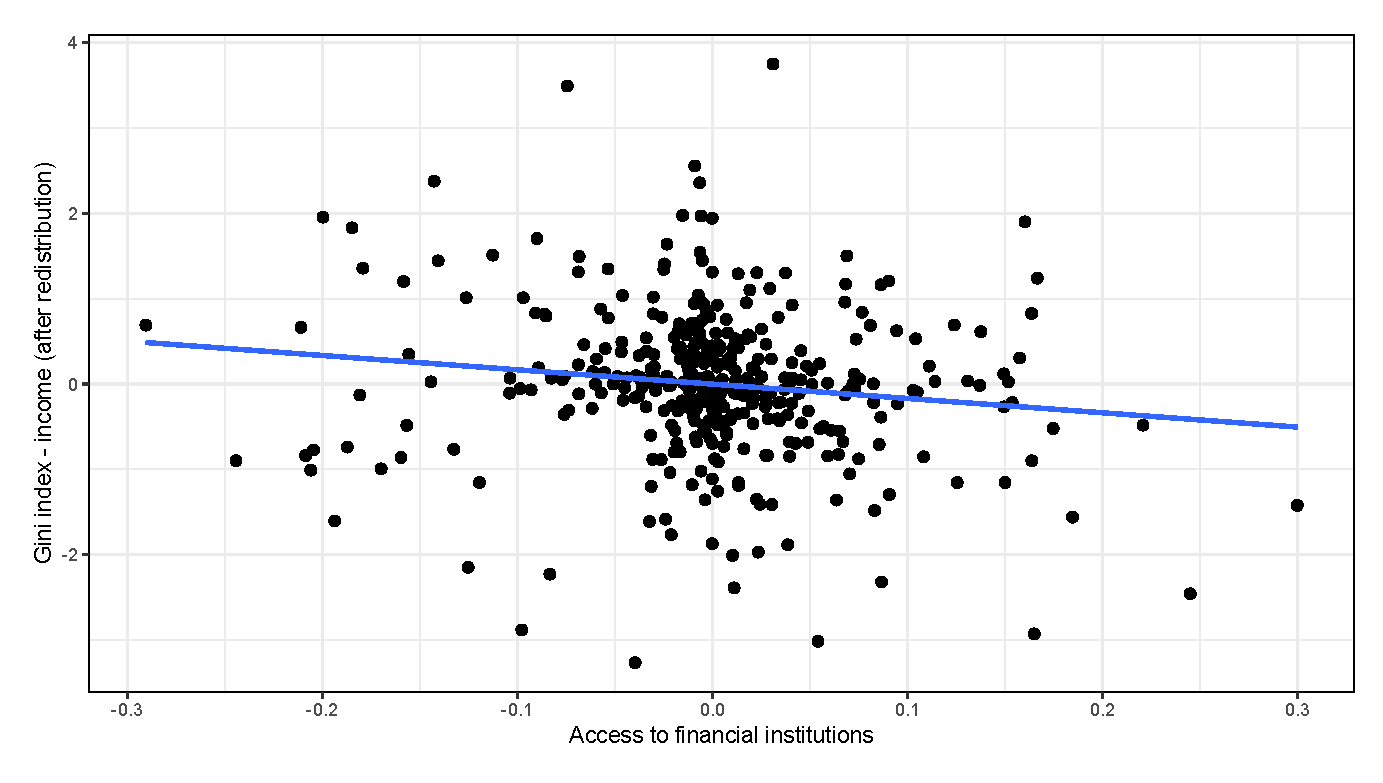
\includegraphics[width=\textwidth, keepaspectratio]{figures/FIAGiniNet_dm}
% \end{figure}

% \begin{figure}
%     \caption{Gini Coefficient and Depth of Financial Institutions}
% 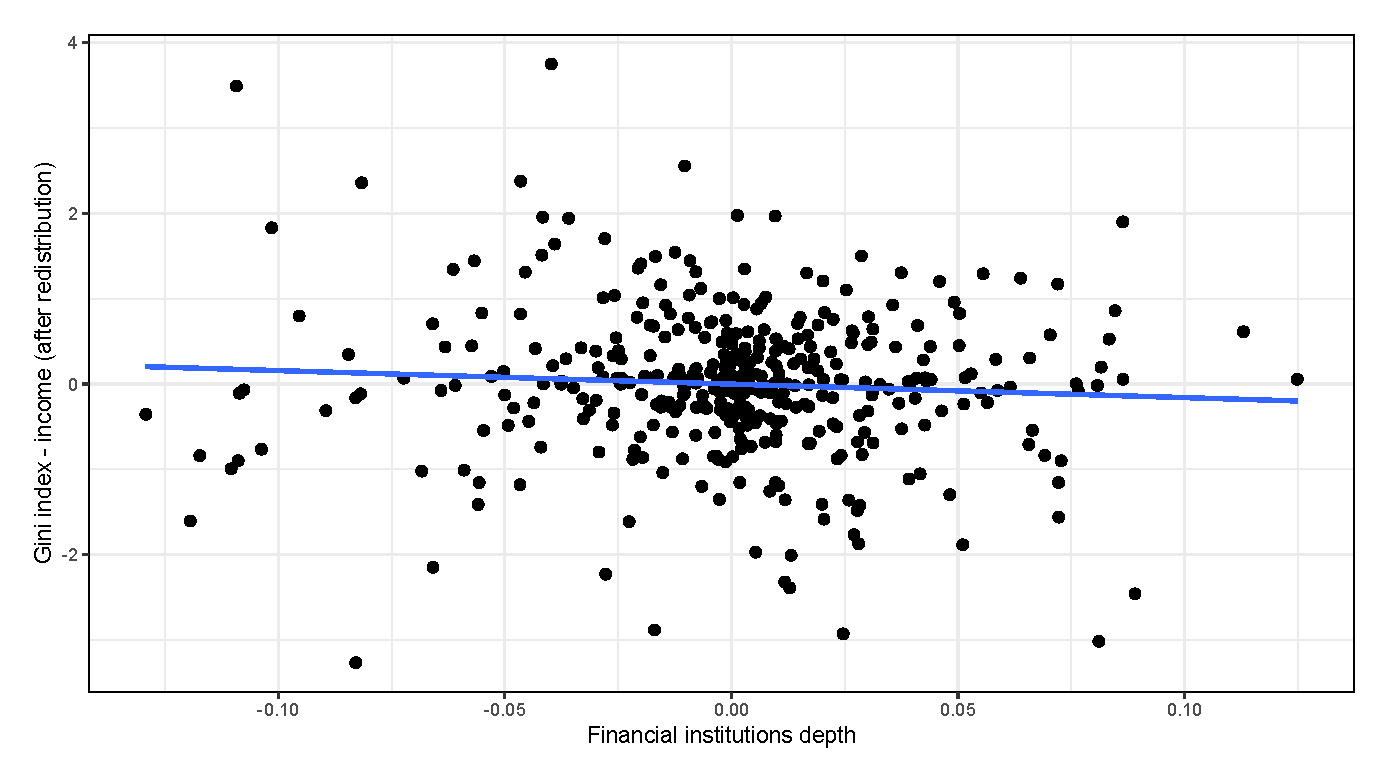
\includegraphics[width=\textwidth, keepaspectratio]{figures/FIDGiniNet_dm}
% \end{figure}

% \begin{figure}
%     \caption{Gini Coefficient and Depth of Financial Markets}
% 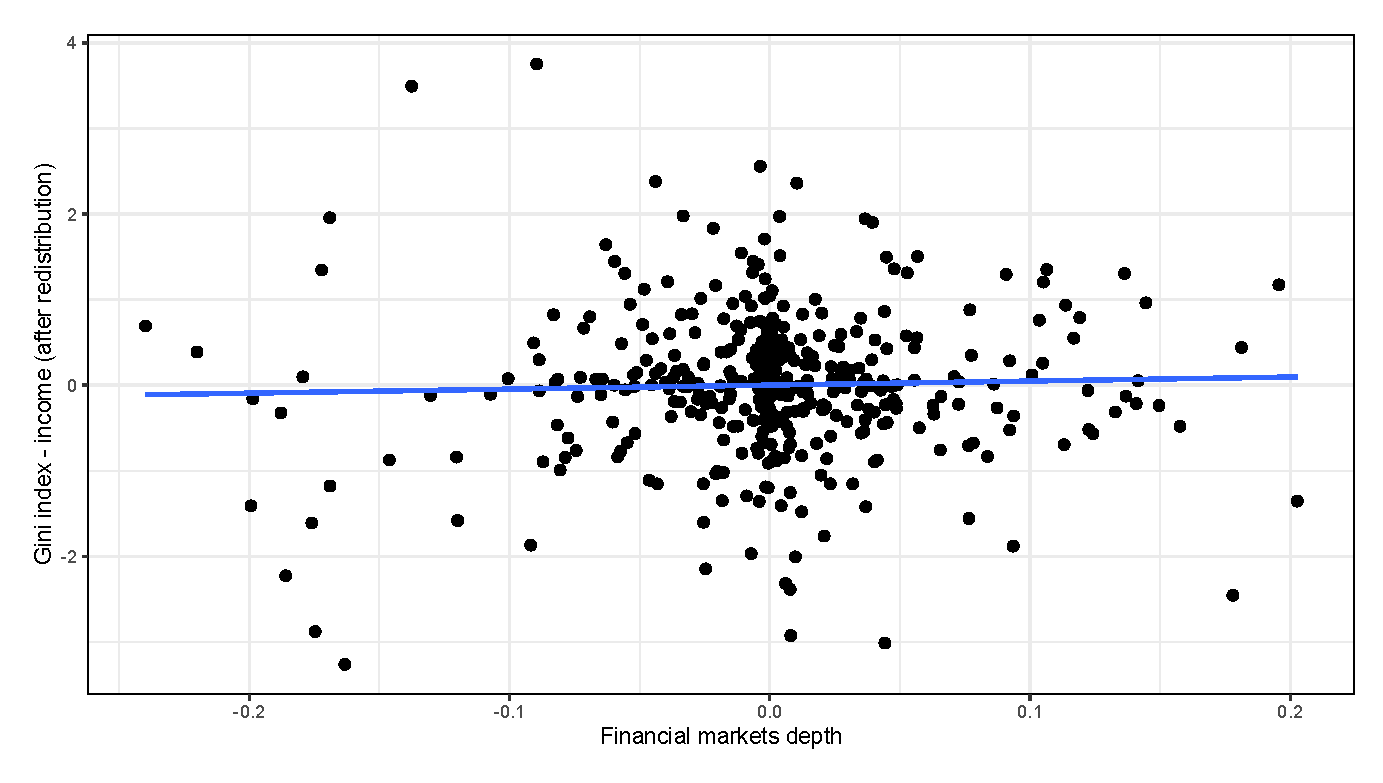
\includegraphics[width=\textwidth, keepaspectratio]{figures/FMDGiniNet_dm}
% \end{figure}

% \begin{figure}
%     \caption{Gini Coefficient and Government Expenditures}
% 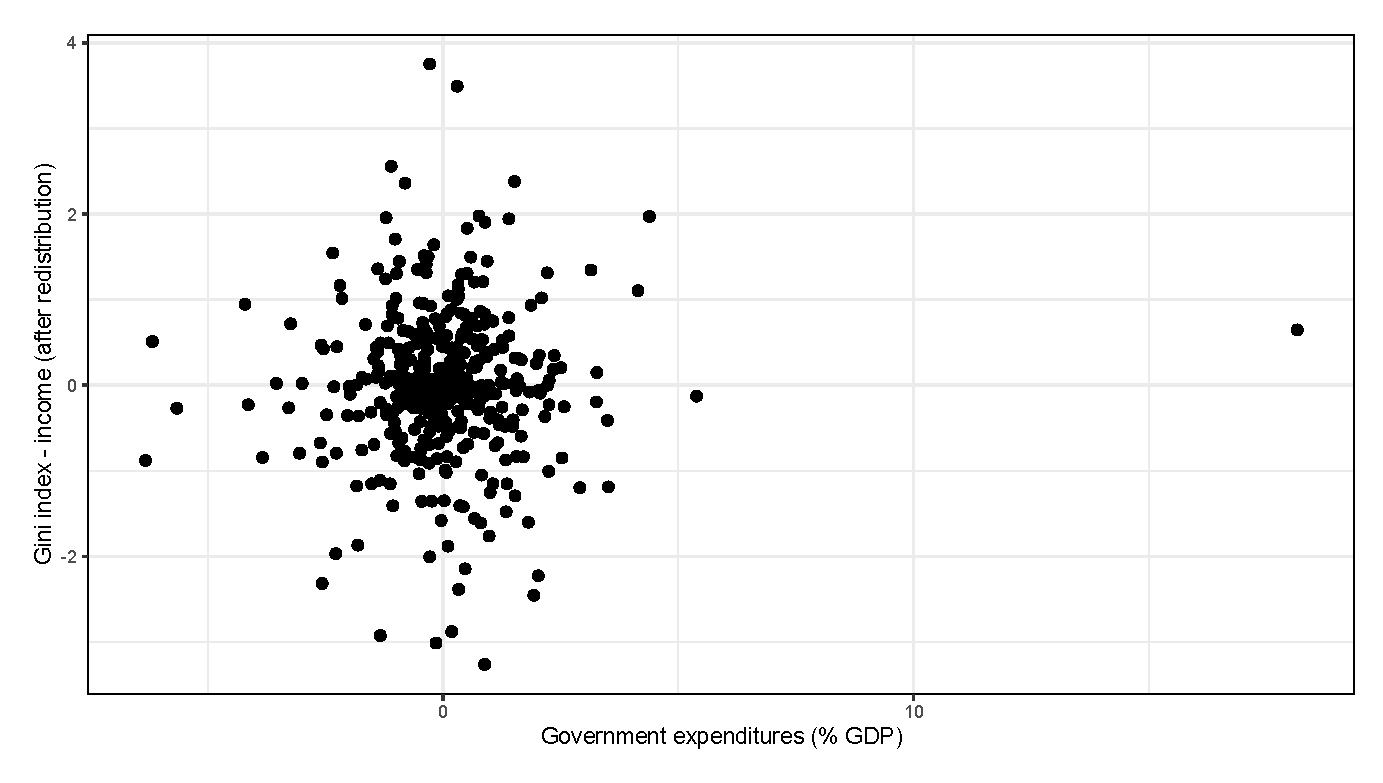
\includegraphics[width=\textwidth, keepaspectratio]{figures/GovExpGiniNet_dm}
% \end{figure}

% \begin{figure}
%     \caption{Gini Coefficient and Mortality}
% 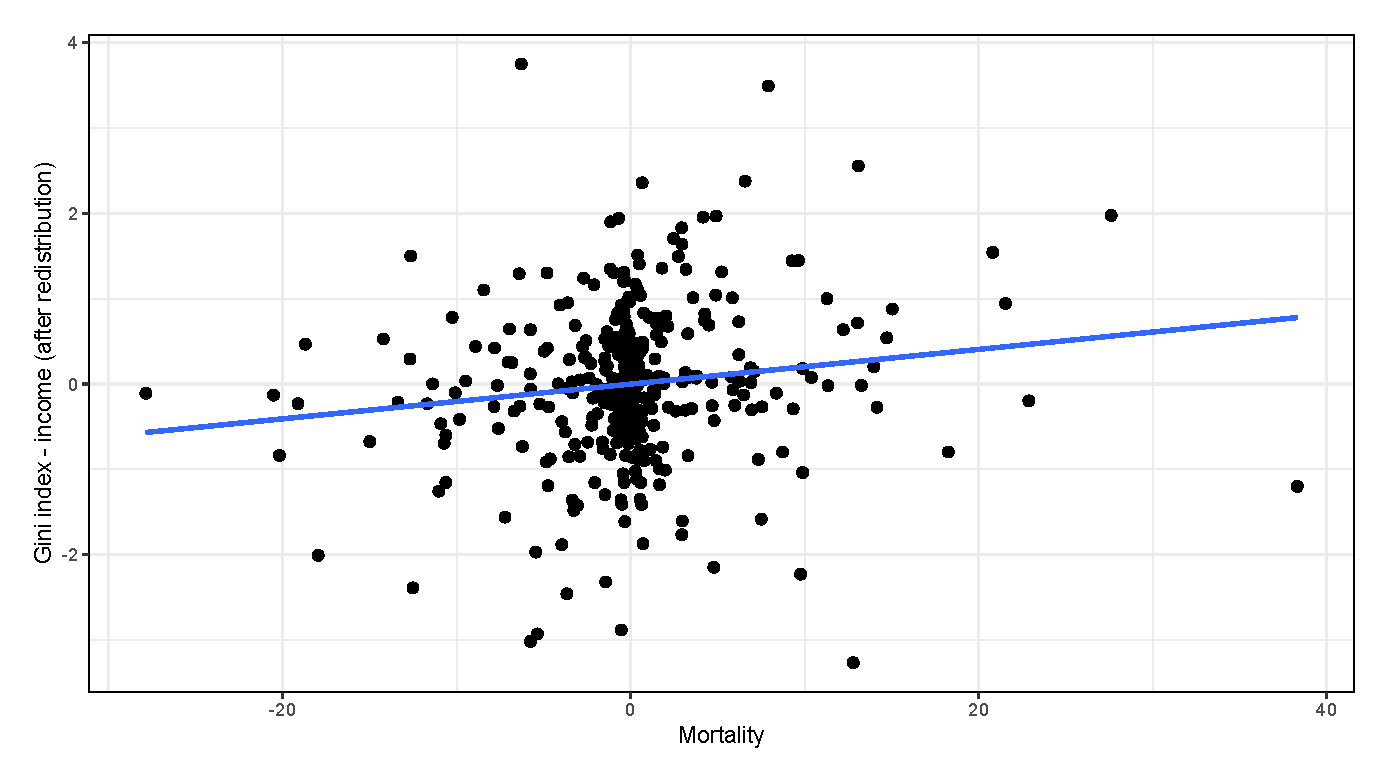
\includegraphics[width=\textwidth, keepaspectratio]{figures/MortGiniNet_dm}
% \end{figure}

% \begin{figure}
%     \caption{Gini Coefficient and \ac{gdp} per capita}
% 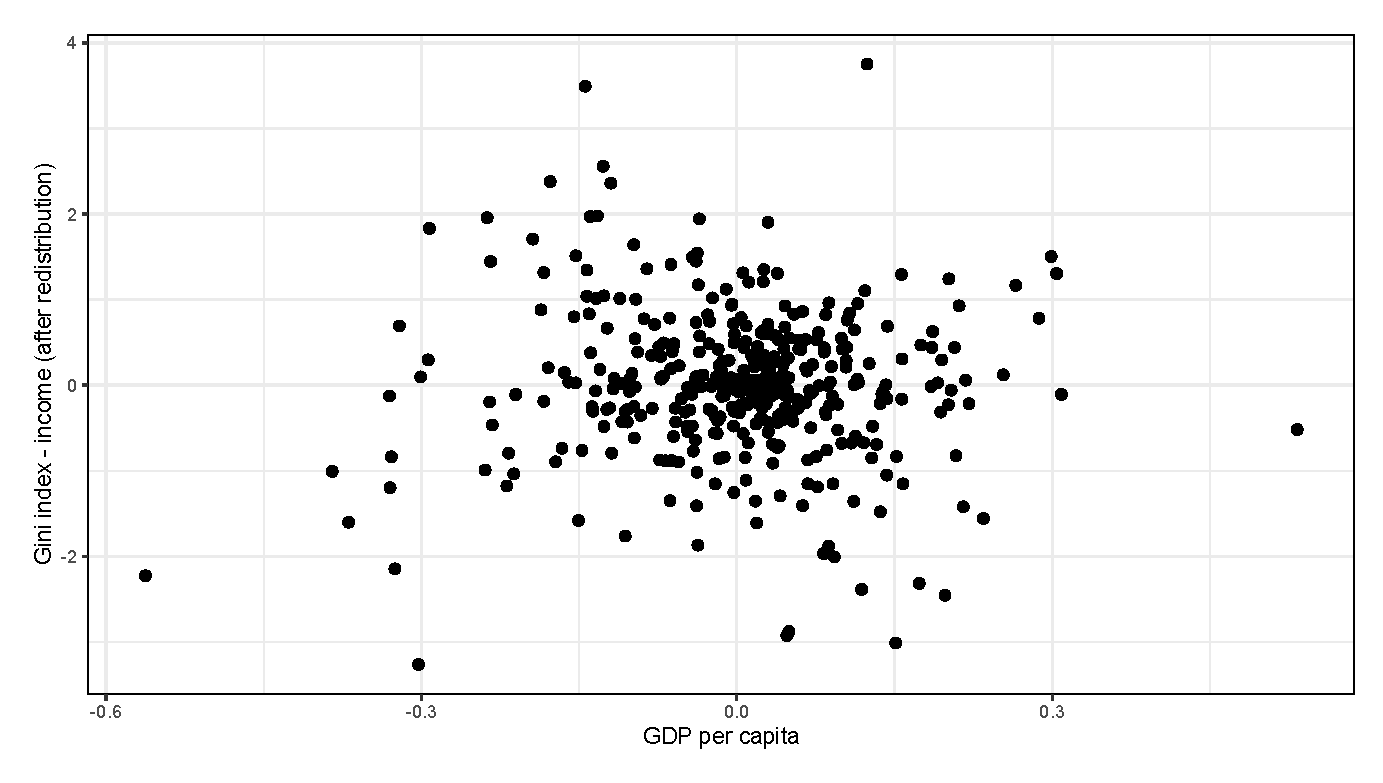
\includegraphics[width=\textwidth, keepaspectratio]{figures/GDPGiniNet_dm}
% \end{figure}

% \begin{figure}
%     \caption{Gini Coefficient and Rule of Law}
% 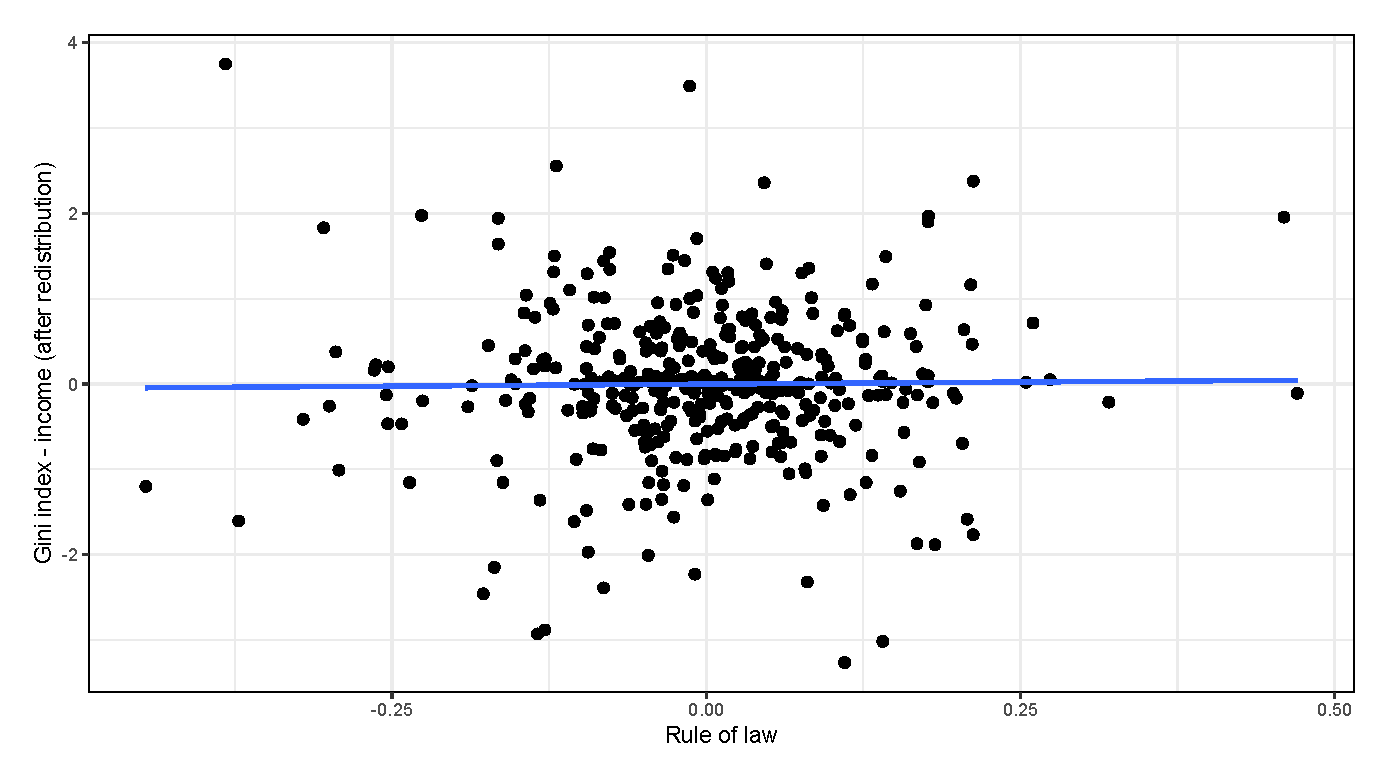
\includegraphics[width=\textwidth, keepaspectratio]{figures/RuleLawGiniNet_dm}
% \end{figure}

% \begin{figure}
%     \caption{Gini Coefficient and Inflation}
% 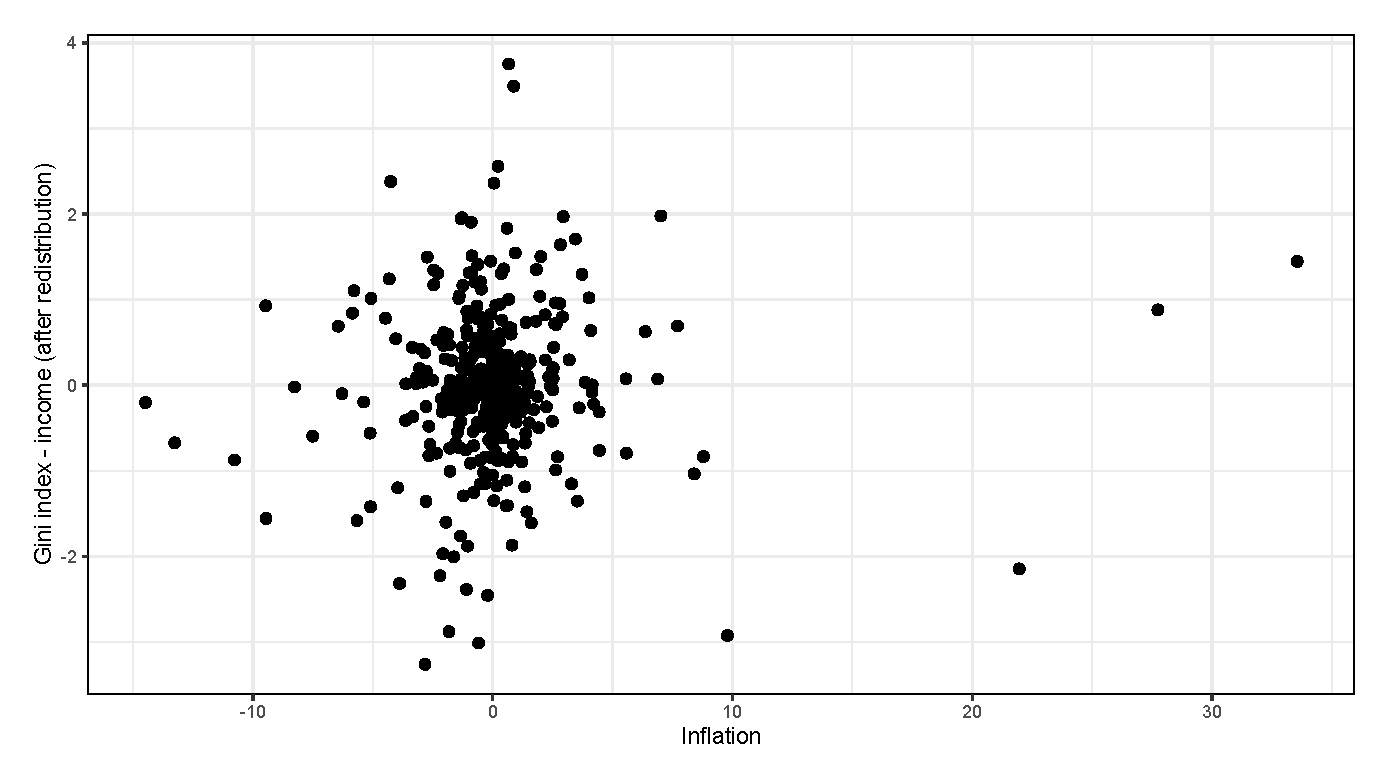
\includegraphics[width=\textwidth, keepaspectratio]{figures/InflGiniNet_dm}
% \end{figure}

% \begin{figure}
%     \caption{Gini Coefficient and Equipment Investment}
% 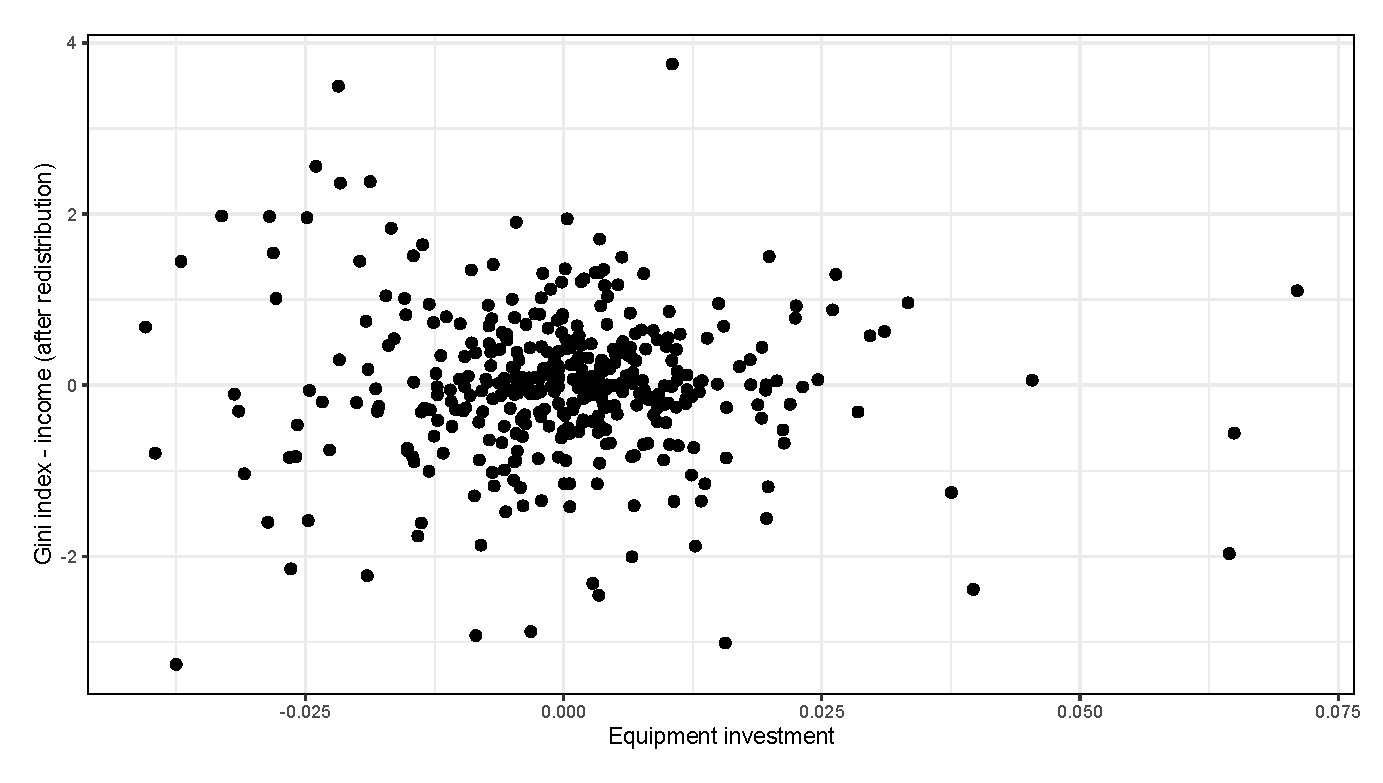
\includegraphics[width=\textwidth, keepaspectratio]{figures/EquipIGiniNet_dm}
% \end{figure}

% \begin{figure}
%     \caption{Gini Coefficient and Trade Openness}
% 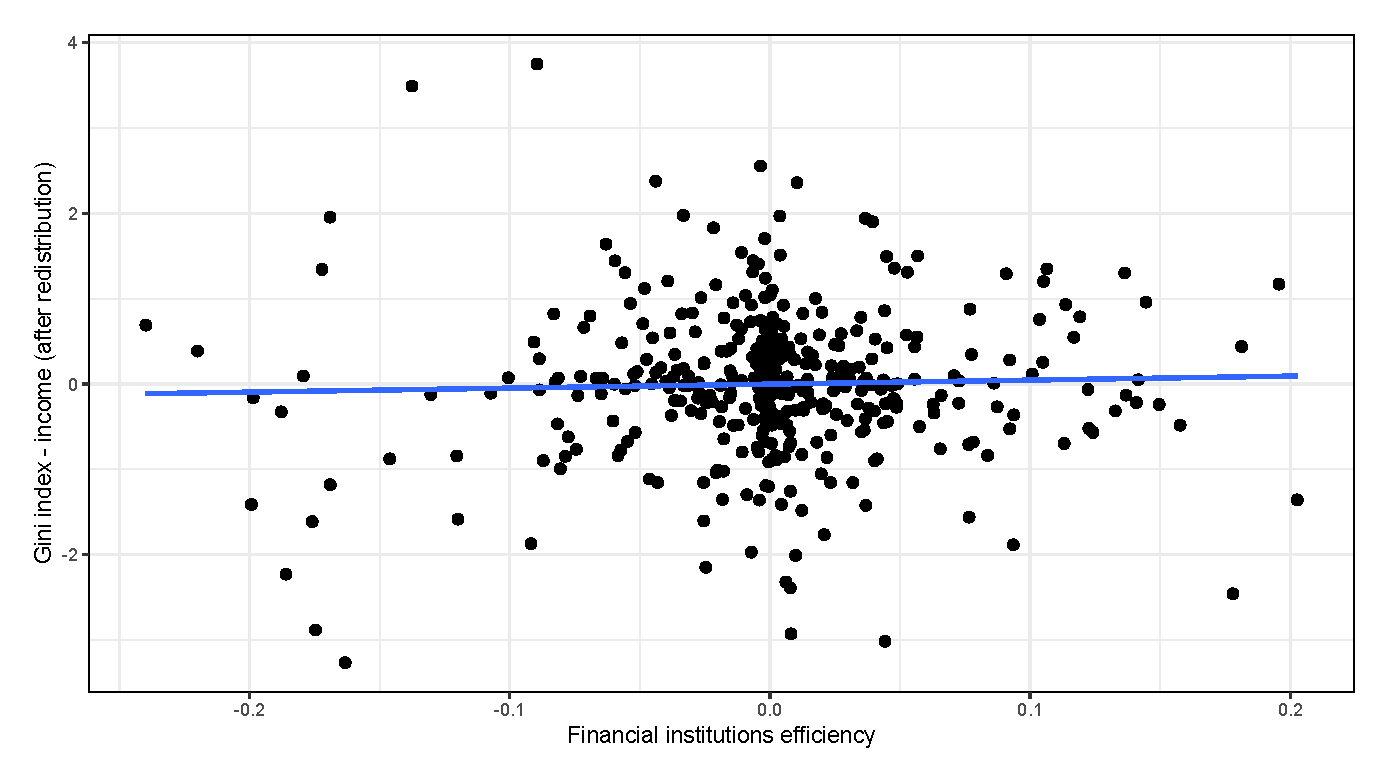
\includegraphics[width=\textwidth, keepaspectratio]{figures/TradeOpenGiniNet_dm}
% \end{figure}

% \begin{figure}
%     \caption{Gini Coefficient and Financial Development Indicators}
% 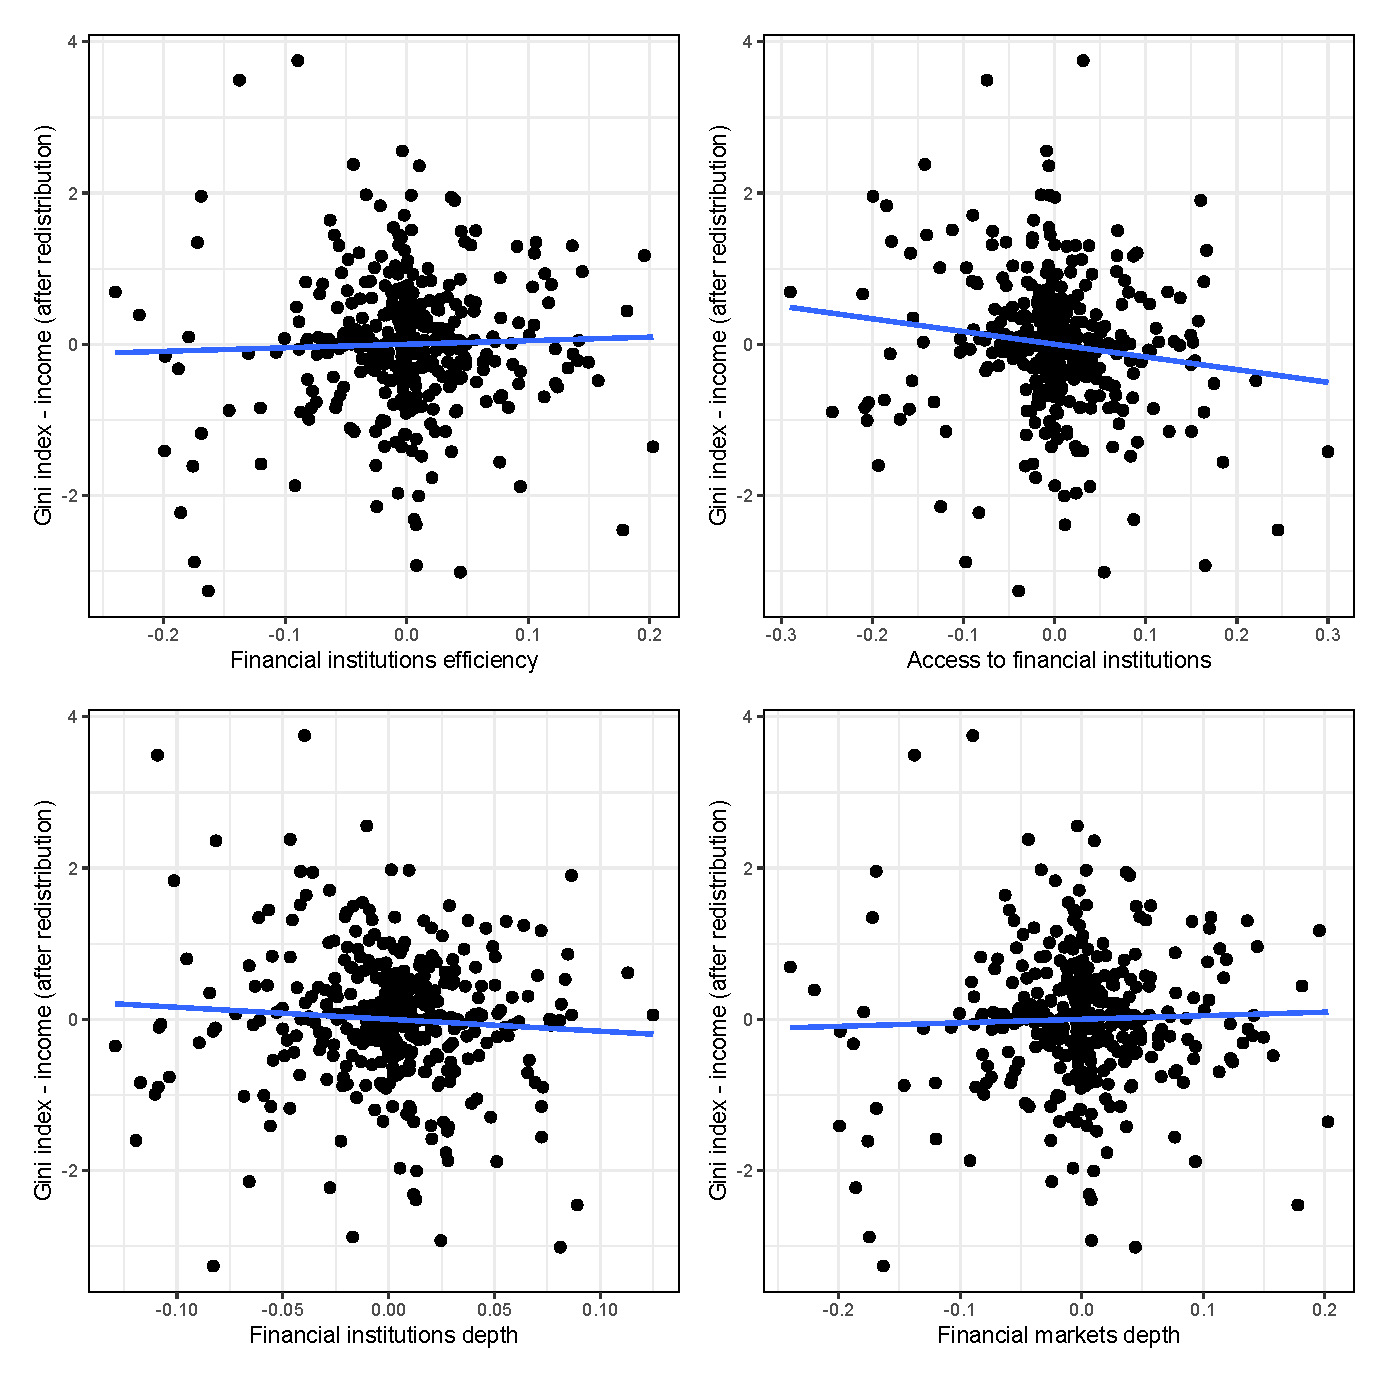
\includegraphics[width=\textwidth, keepaspectratio]{figures/plots_findev_gini_dm}
% \end{figure}

%
%
\section{Methodology}
% \label{sec:meth}

\section{Results}
% \label{sec:results}
The benefits of capital markets liberalization seem to be concentrated to the top of the income distribution. Top quintile of the distribution accrues nearly all of the income growth following the liberalization while the share of middle three quantiles decreases and the bottom remains unaffected \citep{das2003income}.

\citet{kroszneretal2007} show that financial crises have relative more severe impact on the sectors which depend more on external financing. The consequences of crises on firms relate to institutional environment and materialize through lower production capacity and competition.

\section{Conclusion}
\label{sec:conclusion}

\clearpage
%
\bibliographystyle{chicagoa}
\bibliography{literature}
%
% \clearpage
%
% \appendix
% \section{Appendix}
% \label{sec:app}

\renewcommand{\thesection}{A\arabic{section}}%
\renewcommand{\thetable}{A\arabic{table}}%
\renewcommand{\thefigure}{A\arabic{figure}}%
\renewcommand{\theequation}{A\arabic{eq}} 

\end{document}